% PointNet surrogate architecture (InterpretTME). Build:
%   pdflatex surrogate-architecture.tex
%   pdftoppm -png -r 300 -singlefile surrogate-architecture.pdf ../public/images/projects/surrogate-pointnet-architecture
\documentclass[tikz,border=6pt]{standalone}
\usepackage[T1]{fontenc}
\usepackage{helvet}
\usepackage{sansmath}
\renewcommand{\familydefault}{\sfdefault}
\sansmath
\usetikzlibrary{arrows.meta,positioning,fit,backgrounds,calc}

\definecolor{ink}{HTML}{1F2933}
\definecolor{muted}{HTML}{5F6B7A}
\definecolor{dataF}{HTML}{F1F3F5}  \definecolor{dataB}{HTML}{8A94A3}
\definecolor{mlpF}{HTML}{DCE8F5}   \definecolor{mlpB}{HTML}{3B6EA5}
\definecolor{attF}{HTML}{FBE6CF}   \definecolor{attB}{HTML}{C9731A}
\definecolor{aggF}{HTML}{DDEFDD}   \definecolor{aggB}{HTML}{3F8A4A}
\definecolor{grpF}{HTML}{FAFBFC}   \definecolor{grpB}{HTML}{C5CCD6}

\begin{document}
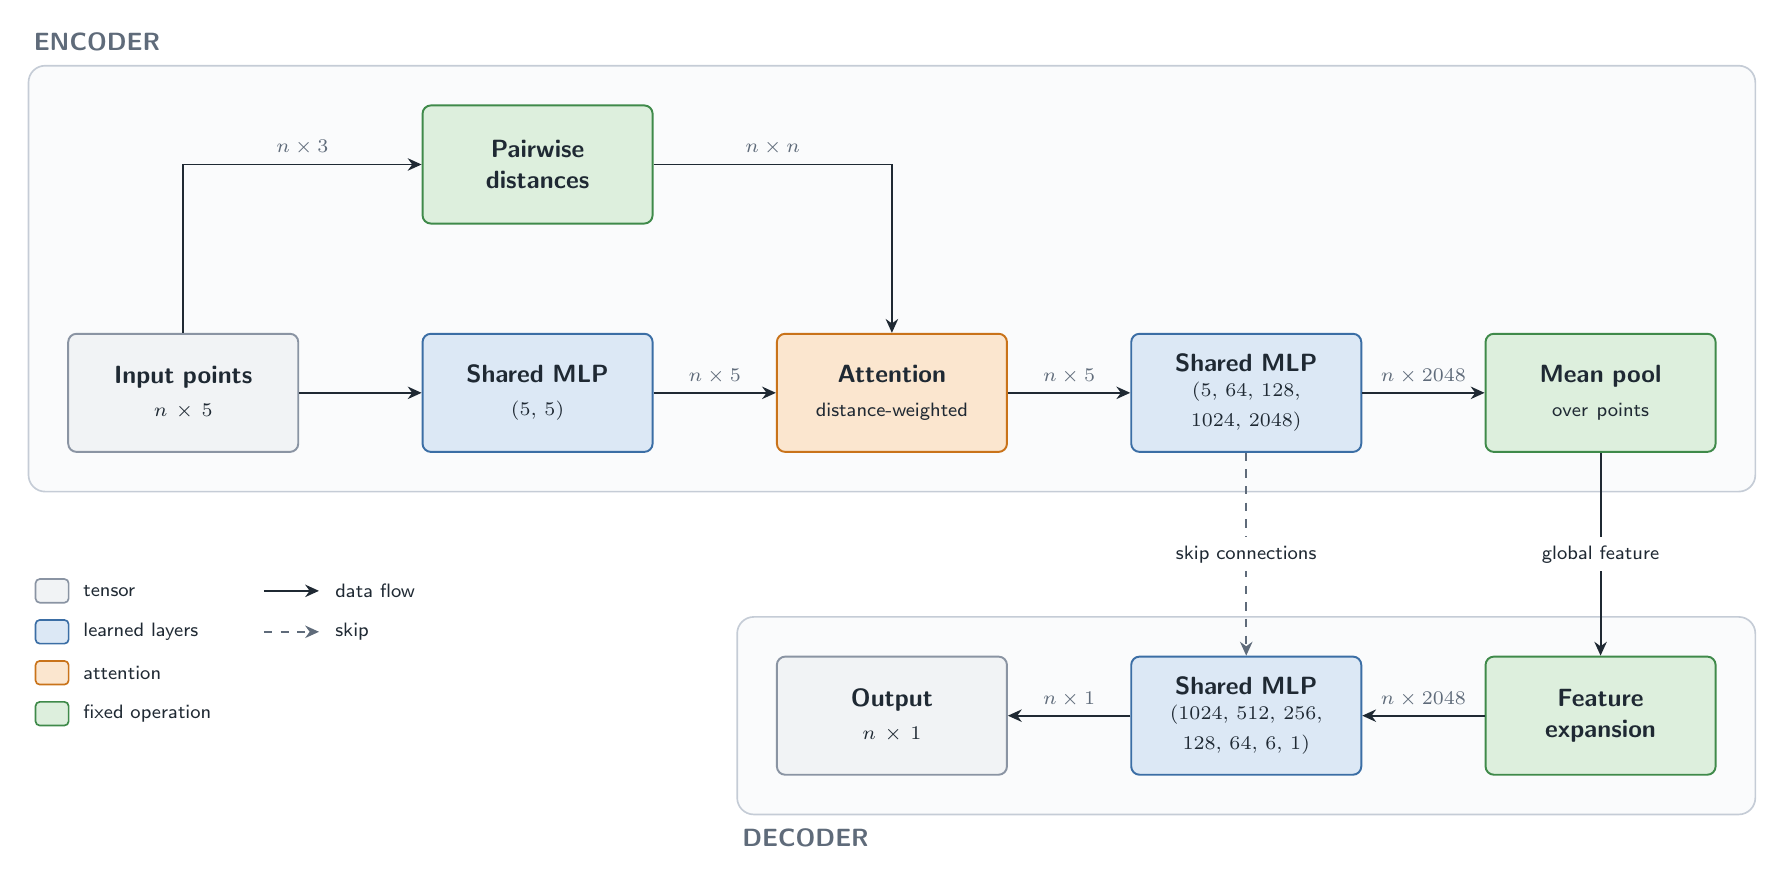
\begin{tikzpicture}[
  font=\small, text=ink, >={Stealth[length=5pt,width=4.5pt]},
  box/.style={draw, line width=0.7pt, rounded corners=3pt, align=center,
              text width=2.5cm, minimum height=1.5cm, inner sep=6pt},
  data/.style={box, fill=dataF, draw=dataB},
  mlp/.style={box, fill=mlpF, draw=mlpB},
  att/.style={box, fill=attF, draw=attB},
  agg/.style={box, fill=aggF, draw=aggB},
  flow/.style={->, line width=0.7pt, draw=ink},
  skip/.style={->, line width=0.7pt, draw=muted, dashed},
  dim/.style={font=\scriptsize, text=muted, inner sep=3pt},
  tag/.style={font=\scriptsize, text=ink, fill=white, inner sep=3pt},
  sub/.style={font=\scriptsize},
]
\def\dx{4.5}

% ---------- encoder ----------
\node[data] (in)   at (0,0)       {\textbf{Input points}\\[1pt]{\scriptsize $n \times 5$}};
\node[mlp]  (mlp1) at (\dx,0)     {\textbf{Shared MLP}\\[1pt]{\scriptsize $(5,\,5)$}};
\node[att]  (att)  at (2*\dx,0)   {\textbf{Attention}\\[1pt]{\scriptsize distance-weighted}};
\node[mlp]  (mlp2) at (3*\dx,0)   {\textbf{Shared MLP}\\[1pt]{\scriptsize $(5,\,64,\,128,$\\ $1024,\,2048)$}};
\node[agg]  (pool) at (4*\dx,0)   {\textbf{Mean pool}\\[1pt]{\scriptsize over points}};
\node[agg]  (dist) at (\dx,2.9)   {\textbf{Pairwise}\\\textbf{distances}};

\draw[flow] (in) -- (mlp1);
\draw[flow] (mlp1) -- node[dim,above] {$n \times 5$} (att);
\draw[flow] (att)  -- node[dim,above] {$n \times 5$} (mlp2);
\draw[flow] (mlp2) -- node[dim,above] {$n \times 2048$} (pool);
\draw[flow] (in.north) |- node[dim,above,pos=0.75] {$n \times 3$} (dist.west);
\draw[flow] (dist.east) -| node[dim,above,pos=0.25] {$n \times n$} (att.north);

% ---------- decoder ----------
\node[agg]  (exp)  at (4*\dx,-4.1) {\textbf{Feature}\\\textbf{expansion}};
\node[mlp]  (mlp3) at (3*\dx,-4.1) {\textbf{Shared MLP}\\[1pt]{\scriptsize $(1024,\,512,\,256,$\\ $128,\,64,\,6,\,1)$}};
\node[data] (out)  at (2*\dx,-4.1) {\textbf{Output}\\[1pt]{\scriptsize $n \times 1$}};

\draw[flow] (pool) -- node[tag,pos=0.5] {global feature} (exp);
\draw[flow] (exp)  -- node[dim,above] {$n \times 2048$} (mlp3);
\draw[flow] (mlp3) -- node[dim,above] {$n \times 1$} (out);
\draw[skip] (mlp2) -- node[tag,pos=0.5] {skip connections} (mlp3);

% ---------- groups ----------
\begin{scope}[on background layer]
  \node[draw=grpB, fill=grpF, line width=0.6pt, rounded corners=6pt,
        inner xsep=14pt, inner ysep=14pt, fit=(in)(dist)(pool)] (enc) {};
  \node[draw=grpB, fill=grpF, line width=0.6pt, rounded corners=6pt,
        inner xsep=14pt, inner ysep=14pt, fit=(out)(exp)] (dec) {};
\end{scope}
\node[anchor=south west, font=\small\bfseries, text=muted, inner sep=2pt]
  at ([yshift=3pt]enc.north west) {ENCODER};
\node[anchor=north west, font=\small\bfseries, text=muted, inner sep=2pt]
  at ([yshift=-3pt]dec.south west) {DECODER};

% ---------- legend ----------
\begin{scope}[shift={($(enc.south west)+(0.1,-1.25)$)}]
  \foreach \i/\f/\b/\t in {0/dataF/dataB/tensor, 1/mlpF/mlpB/learned layers,
                           2/attF/attB/attention, 3/aggF/aggB/fixed operation} {
    \node[draw=\b, fill=\f, line width=0.6pt, rounded corners=1.5pt,
          minimum width=0.42cm, minimum height=0.3cm, inner sep=0pt] at (0.21,-0.52*\i) {};
    \node[anchor=west, font=\scriptsize, text=ink, inner sep=0pt] at (0.6,-0.52*\i) {\t};
  }
  \draw[flow] (2.9,0) -- (3.6,0);
  \node[anchor=west, font=\scriptsize, inner sep=0pt] at (3.8,0) {data flow};
  \draw[skip] (2.9,-0.52) -- (3.6,-0.52);
  \node[anchor=west, font=\scriptsize, inner sep=0pt] at (3.8,-0.52) {skip};
\end{scope}
\end{tikzpicture}
\end{document}
